\chapter{空间相干与强度干涉}
\label{chap:05}

\begin{chapteropening}
第 \ref{chap:04} 章讨论的是同一束光在不同时间是否相关。现在把问题换成空间版本：两台望远镜相隔几十米、几百米甚至几公里，它们看到的是同一颗星，但记录到的强度涨落还会不会同步？如果同步，说明这条基线对应的角尺度上天体还没有被完全分辨；如果不同步，说明天空亮度结构已经在这个空间频率上把相干性洗掉了。

这就是空间强度干涉的核心。van Cittert--Zernike 定理把天空亮度变成复可见度，Hanbury Brown--Twiss 相关器把强度涨落变成 \(|V|^2\)，Narrabri 恒星强度干涉仪证明了这可以测恒星角直径。现代 VERITAS、MAGIC、H.E.S.S. 和 CTAO 这类大气 Cherenkov 望远镜阵列又让这个思想重新变得实际，因为它们天然拥有大口径、快速探测器和长基线 \citep{1938Phy.....5..785Z,1939Phy.....6.1129V,1956Natur.177...27B,1957RSPSA.242..300B,1958RSPSA.248..222B,1967MNRAS.137..375H,1967MNRAS.137..393H,1974iiia.book.....H,2006ApJ...649..399L,2013APh....43..331D,2020NatAs...4.1164A,2024MNRAS.529.4387A}。
\end{chapteropening}

\section{基线为什么会选择一个角尺度}

先不谈相关器，只看一件几何事实。来自天空不同方向的平面波，到达两台望远镜时走过的路程不同。两台望远镜的位置为 \(\mathbf{x}_1\) 和 \(\mathbf{x}_2\)，把它们的间隔投影到垂直视线的天空平面，得到
\[
  \mathbf{B}_\perp=\mathbf{x}_{2,\perp}-\mathbf{x}_{1,\perp}.
\]
对于相对于相位中心的小角度方向 \((l,m)\)，路径差近似是 \(B_x l+B_y m\)。长度差除以波长再乘 \(2\pi\)，就是这个方向给两台望远镜带来的相位差。因此同一条物理基线在不同波长下对应不同的空间频率：
\begin{equation}
  u=\frac{B_x}{\lambda},
  \qquad
  v=\frac{B_y}{\lambda}.
  \label{eq:ch05-uv}
\end{equation}
\begin{formulaexplain}
\(B_x,B_y\) 是投影基线在天空平面的两个分量；\(\lambda\) 是观测波长；\(u,v\) 是以波长为单位的空间频率。它说明同一条基线在短波长下采样更细的角结构。
\end{formulaexplain}
\(B_x,B_y\) 和 \(\lambda\) 都用米，所以 \(u,v\) 是无量纲的“波长数”。若 \(B=100\,{\rm m}\)、\(\lambda=500\,{\rm nm}\)，则 \(B/\lambda=2\times10^8\)。这不是角分辨率本身，而是 Fourier 平面上的采样位置；把它倒过来，才得到约 \(\lambda/B\simeq1\,{\rm mas}\) 的角尺度。

两台望远镜之间的一阶空间相干度定义为
\begin{equation}
  \gamma_{12}^{(1)}
  =
  \frac{\left\langle E_1^\ast(t)E_2(t)\right\rangle}
  {\sqrt{\left\langle |E_1(t)|^2\right\rangle
  \left\langle |E_2(t)|^2\right\rangle}} .
  \label{eq:ch05-gamma12}
\end{equation}
\begin{formulaexplain}
\(E_1,E_2\) 是两台望远镜接收的电场；分子是跨望远镜的场相关，分母用各自强度归一化。\(\gamma_{12}^{(1)}\) 是复相干度，模给相干强弱，相位给 Fourier 相位。
\end{formulaexplain}
\(\gamma_{12}^{(1)}\) 是复数。它的模表示两台望远镜接收到的场有多相干，复相位记录 Fourier 相位。振幅干涉仪把两束光用延迟线合到一起，直接测这个复可见度或至少测它的条纹相位与可见度；强度干涉仪不在光学上合束，而是在探测之后比较两路强度涨落，所以最直接得到的是 \(|\gamma_{12}^{(1)}|^2\)。

van Cittert--Zernike 定理说明，远场非相干源的这个空间相干度就是天空亮度的归一化 Fourier 分量：
\begin{equation}
  \gamma^{(1)}(u,v)
  =
  \frac{
    \int I_\nu(l,m)\,
    \exp[-2\pi i(ul+vm)]\,dl\,dm
  }{
    \int I_\nu(l,m)\,dl\,dm
  } .
  \label{eq:ch05-vcz}
\end{equation}
\begin{formulaexplain}
\(I_\nu(l,m)\) 是天空亮度，\(l,m\) 是小角度坐标；指数项把每个方向映射到空间频率 \(u,v\) 的相位；分母是总通量。VCZ 定理把天空图像变成归一化复可见度。
\end{formulaexplain}
\(I_\nu(l,m)\) 是方向 \((l,m)\) 上的比强度，常用单位是 \({\rm erg\,s^{-1}\,cm^{-2}\,Hz^{-1}\,sr^{-1}}\) 或等效的光子谱亮度；\(l,m\) 是小角度坐标，按弧度处理；分母把总通量归一化，因此 \(\gamma^{(1)}(0,0)=1\)。这条式子的物理含义很直接：短基线只看天空亮度的粗结构，长基线看细结构；若源在某个角尺度上很大，长基线上的相干度就下降。

式 \eqref{eq:ch05-vcz} 也有边界。源内部各点在发射时要彼此非相干；带宽不能宽到让不同 \(\lambda\) 对应的 \(u,v\) 混在一起；小视场近似要足够好，使 \(w\)-term 可以忽略；观测时间内源结构不能在相关积累时显著变化。对普通热星和窄带蓝光强度干涉，这些条件通常可控；对快速瞬变、宽带成像或大视场目标，就必须重新检查 \citep{1938Phy.....5..785Z,1939Phy.....6.1129V,2000stop.book.....G,2007itcp.book.....W}。

\begin{figure}[tbp]
\centering
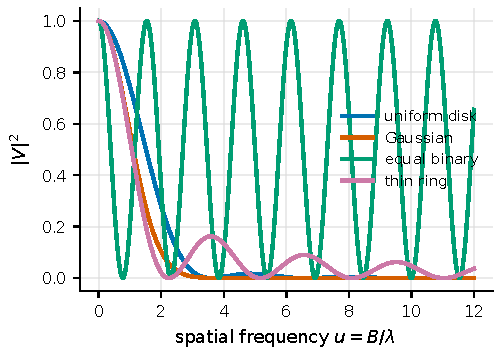
\includegraphics[width=0.88\linewidth]{figures/generated/chapter_05/ch05_vcz_visibility_models.pdf}
\caption{不同天空亮度模型在 \(|V|^2\) 空间留下不同结构。均匀圆盘有 Bessel 型零点，Gaussian 源平滑下降，等亮双星产生余弦振荡，薄环产生更密的振荡。强度干涉直接给出这些曲线的模平方，而不是复可见度本身。}
\label{fig:ch05-vcz-models}
\end{figure}

\section{从可见度曲线读出恒星角直径}

把 VCZ 定理用于恒星，最简单的模型是均匀圆盘。假设恒星角直径为 \(\theta\)，表面亮度在圆盘内为常数，在圆盘外为零。圆对称的 Fourier 变换给出
\begin{equation}
  V(B)=\frac{2J_1(x)}{x},
  \qquad
  x=\frac{\pi\theta B}{\lambda},
  \label{eq:ch05-uniform-disk}
\end{equation}
\begin{formulaexplain}
\(V(B)\) 是均匀圆盘的可见度；\(J_1\) 是一阶 Bessel 函数；\(\theta\) 是角直径，\(B\) 是投影基线。无量纲量 \(x\) 决定圆盘在该基线上被分辨到什么程度。
\end{formulaexplain}
其中 \(J_1\) 是一阶 Bessel 函数，\(\theta\) 用弧度，\(B\) 是投影基线长度，\(\lambda\) 是观测波长。式子里的无量纲组合 \(x=\pi\theta B/\lambda\) 是最重要的量：同一颗星在更长基线或更短波长下更容易被分辨，同一条基线对更大的角直径也更敏感。

均匀圆盘的第一个零点满足 \(x=3.8317\)，因此
\begin{equation}
  B_0\simeq \frac{1.22\,\lambda}{\theta}.
  \label{eq:ch05-first-null}
\end{equation}
\begin{formulaexplain}
\(B_0\) 是均匀圆盘可见度的第一零点基线；\(\lambda\) 是波长，\(\theta\) 是角直径。它给出“刚好分辨到第一个暗纹”所需的基线尺度。
\end{formulaexplain}
\(B_0\) 的单位是米。取 VERITAS 和 MAGIC 常用的蓝光波段 \(\lambda=416\,{\rm nm}\)，若 \(\theta=1\,{\rm mas}=4.848\times10^{-9}\,{\rm rad}\)，第一个零点约 \(105\,{\rm m}\)；若 \(\theta=0.5\,{\rm mas}\)，需要约 \(210\,{\rm m}\)；若 \(\theta=0.2\,{\rm mas}\)，需要约 \(520\,{\rm m}\)。这解释了为什么 Narrabri 的 10--188 m 基线能测亮的亚毫角秒恒星，而公里级 CTAO 阵列有机会进入几十微角秒角尺度 \citep{1967MNRAS.137..375H,1967MNRAS.137..393H,1974MNRAS.167..121H,1974iiia.book.....H,2006ApJ...649..399L,2014SPIE.9146E..0ZD}。

\begin{figure}[tbp]
\centering
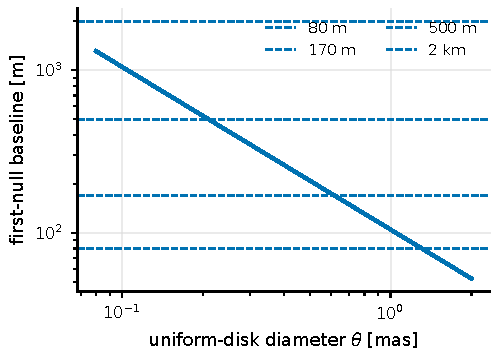
\includegraphics[width=0.86\linewidth]{figures/generated/chapter_05/ch05_uniform_disk_resolution.pdf}
\caption{均匀圆盘在 \(\lambda=416\,{\rm nm}\) 下的第一零点基线。0.5 mas 恒星需要约 210 m 才到第一个零点，0.1 mas 量级目标需要公里级基线；这正是 Cherenkov 阵列对蓝光强度干涉有吸引力的原因。}
\label{fig:ch05-uniform-disk-resolution}
\end{figure}

实际观测不会只问“零点在哪里”。最有信息的往往是第一 lobe 的下降区：短基线处 \(|V|^2\simeq1\)，不同角直径曲线几乎重合；零点以后 \(|V|^2\) 很低，系统误差和背景容易主导；下降区既有较大信号，又对 \(\theta\) 敏感。因此设计观测时通常要先画出目标模型的 \(|V(B)|^2\) 和不同角直径的差异，选择能覆盖下降区和零点附近的投影基线。

均匀圆盘也只是第一模型。热星有 limb darkening，快速自转星有赤道鼓包和 gravity darkening，Be 星有盘，双星有两个亮度中心，Cepheid 会随相位改变半径。均匀圆盘直径 \(\theta_{\rm UD}\) 常是便于比较的中间量；要得到 limb-darkened 直径 \(\theta_{\rm LD}\)，需要大气模型和波段响应。VERITAS 对 \(\beta\) CMa 和 \(\epsilon\) Ori 的首批四望远镜强度干涉结果给出 \(\theta_{\rm UD}=0.523\pm0.017\,{\rm mas}\) 和 \(0.631\pm0.017\,{\rm mas}\)，相应 limb-darkened 直径为 \(0.542\pm0.018\,{\rm mas}\) 和 \(0.660\pm0.018\,{\rm mas}\) \citep{2020NatAs...4.1164A}。后续 \(\beta\) UMa 观测和 \(\gamma\) Cas 快速自转星观测说明，随着 \(u,v\) 覆盖改善，强度干涉不只测“一个半径”，也能约束方向依赖的 photosphere 形状 \citep{2024ApJ...966...28A,2025ApJ...995..191A}。

\section{HBT 相关器真正测到什么}

前两节讨论的是一阶相干和复可见度。强度干涉真正记录的是两台望远镜的强度涨落是否同步。第 \ref{chap:04} 章的 Siegert 关系 \eqref{eq:ch04-siegert} 用到空间通道时变成
\begin{equation}
  g_{12}^{(2)}(0)-1
  =
  \zeta\,\left|\gamma_{12}^{(1)}\right|^2 .
  \label{eq:ch05-hbt-spatial}
\end{equation}
\begin{formulaexplain}
\(g_{12}^{(2)}(0)-1\) 是零延迟强度相关的超额；\(\zeta\) 是时间响应、带宽、偏振和背景等稀释因子；\(|\gamma_{12}^{(1)}|^2\) 是平方可见度。它是空间 HBT 的核心关系。
\end{formulaexplain}
\(g_{12}^{(2)}(0)-1\) 是两台望远镜零延迟强度相关的 excess；\(\gamma_{12}^{(1)}\) 是同一基线上的一阶空间相干度；\(\zeta\) 收集有限时间响应、光谱带宽、偏振、背景和仪器归一化。对热光或高斯混沌光，\(|\gamma_{12}^{(1)}|^2=|V(B)|^2\)。因此 HBT 不需要把两台望远镜的电场直接合束，却能通过强度涨落的同步程度测可见度模平方。

数据分析中常把这个关系写成观测模型
\begin{equation}
  C_{12}(B)
  \equiv g_{12}^{(2)}(0)-1
  =
  N_0\,f_1 f_2\,|V(B)|^2 ,
  \label{eq:ch05-correlation-model}
\end{equation}
\begin{formulaexplain}
\(C_{12}\) 是观测到的相关峰幅度；\(N_0\) 是零基线仪器响应；\(f_1,f_2\) 是目标光子占比；\(|V|^2\) 是天体结构项。它把仪器、背景和源结构分开。
\end{formulaexplain}
\(C_{12}(B)\) 是基线 \(B\) 上的相关峰幅度；\(N_0\) 是零基线相关幅度，也就是同一光源在没有空间分辨损失时应有的仪器响应后聚束高度；\(f_1,f_2\) 是两台望远镜中目标光子占总计数的比例；\(V(B)\) 是式 \eqref{eq:ch05-vcz} 给出的归一化可见度。这个模型把三个影响分开：天体结构给 \(|V|^2\)，背景给 \(f_1f_2\)，仪器给 \(N_0\)。

若探测器有效时间宽度为 \(\Delta t_{\rm eff}\)，光学带宽为 \(\Delta\nu\)，未分偏振热光的零基线幅度数量级为
\begin{equation}
  N_0\sim \frac{1}{2\,\Delta\nu\,\Delta t_{\rm eff}},
  \qquad
  \Delta\nu\simeq\frac{c\,\Delta\lambda}{\lambda^2}.
  \label{eq:ch05-n0}
\end{equation}
\begin{formulaexplain}
\(N_0\) 是未被空间分辨时的聚束峰高度；\(\Delta\nu\) 是光学频率带宽；\(\Delta t_{\rm eff}\) 是电子有效时间宽度。带宽和时间响应越宽，热光相关峰被平均得越低。
\end{formulaexplain}
这里的 \(1/2\) 可理解为未分辨两个偏振模式的稀释；若只选一个线偏振，偏振因子会不同。对 VERITAS 的 \(\lambda=416\,{\rm nm}\)、\(\Delta\lambda=13\,{\rm nm}\)、\(\Delta t_{\rm eff}\sim4\,{\rm ns}\)，这个估算给 \(N_0\) 为几 \(10^{-6}\)。实际拟合得到 \(N_0=(1.23\pm0.05)\times10^{-6}\) 和 \((1.26\pm0.06)\times10^{-6}\)，说明光学带宽、电子响应和系统效率共同把热光聚束峰压到百万分之一量级 \citep{2020NatAs...4.1164A}。

\begin{figure}[tbp]
\centering
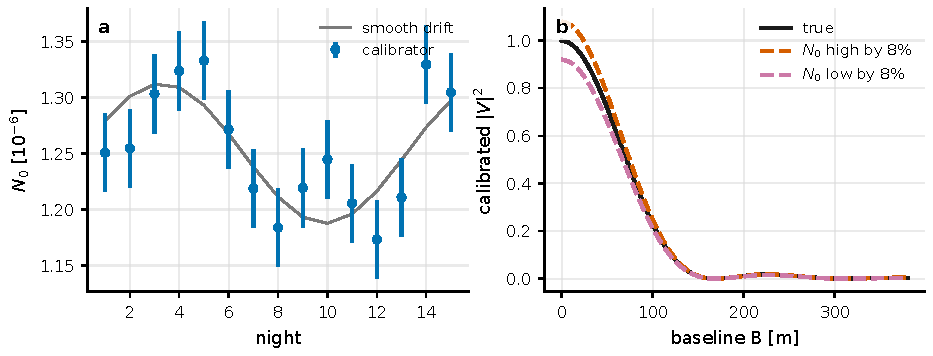
\includegraphics[width=0.92\linewidth]{figures/generated/chapter_05/ch05_zero_baseline_calibration.pdf}
\caption{零基线相关幅度 \(N_0\) 的标定对 \(|V|^2\) 的直接影响。左图示意校准星给出的夜间 \(N_0\) 漂移；右图显示 \(N_0\) 若偏高或偏低 8\%，所有基线上的 \(|V|^2\) 都会被整体拉伸，从而把角直径、边缘昏暗或扁率拟合推向错误值。}
\label{fig:ch05-zero-baseline}
\end{figure}

\begin{figure}[tbp]
\centering
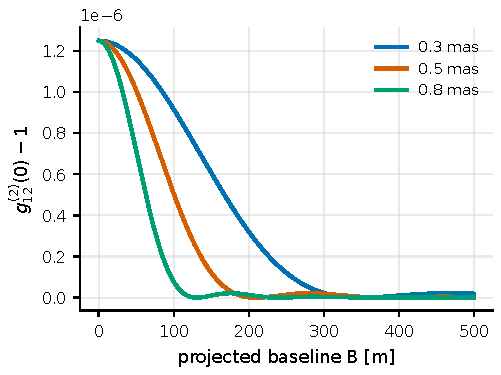
\includegraphics[width=0.86\linewidth]{figures/generated/chapter_05/ch05_sii_signal_vs_baseline.pdf}
\caption{用 \(C_{12}=N_0|V|^2\) 估算的强度干涉信号，\(N_0\) 取 \(1.25\times10^{-6}\) 的现代蓝光系统量级。角直径越大，\(|V|^2\) 越早随基线下降并出现零点；因此同一组基线对 0.8 mas 恒星比对 0.3 mas 恒星更敏感。}
\label{fig:ch05-sii-signal}
\end{figure}

强度干涉的代价是相位缺失。两台望远镜只测 \(|V|^2\)，不能像振幅干涉那样直接得到 Fourier 相位；镜像亮度分布 \(I(-l,-m)\) 与原图有相同的 \(|V|^2\)。它换来的优势是对光学路径的要求大幅降低。振幅干涉需要把光程稳定到波长的一小部分；强度干涉只需要把电子信号对齐到探测响应时间的一小部分。对 \(1\,{\rm GHz}\) 电子带宽，路径误差达到几厘米才会明显降低相关；大气 piston 在光学相位上很致命，但对 ns 量级强度相关几乎不是主噪声源。这也是为什么光学成像质量并非专用干涉仪级别的 Cherenkov 望远镜仍可用于强度干涉 \citep{2006ApJ...649..399L,2008AIPC..984..205L,2013APh....43..331D,2014SPIE.9146E..0ZD}。

\begin{figure}[tbp]
\centering
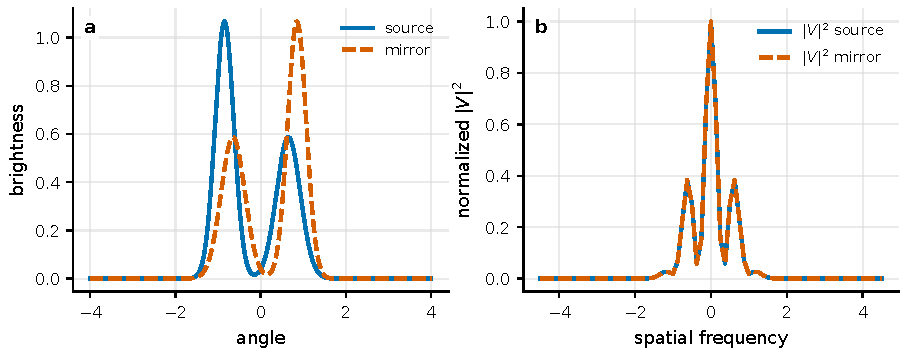
\includegraphics[width=0.92\linewidth]{figures/generated/chapter_05/ch05_phase_ambiguity.pdf}
\caption{只测 \(|V|^2\) 会丢失 Fourier 相位。左图中的源和镜像源亮度分布不同；右图中二者的 \(|V|^2\) 完全重合。强度干涉成像需要二维 \(u,v\) 覆盖、物理先验、三阶相关或相位恢复算法来打破这类退化。}
\label{fig:ch05-phase-ambiguity}
\end{figure}

\section{怎样判断一次观测是否可行}

强度干涉的统计难点来自一个事实：信号幅度很小，而随机符合数很大。Hanbury Brown 的双望远镜强度干涉信噪比常写成
\begin{equation}
  \left(\frac{S}{N}\right)_{\rm rms}
  =
  A\,\alpha\,n\,|\gamma_{12}^{(1)}|^2
  \left(\frac{\Delta f\,T}{2}\right)^{1/2}.
  \label{eq:ch05-snr}
\end{equation}
\begin{formulaexplain}
\(A\) 是收集面积，\(\alpha\) 是探测效率，\(n\) 是光子谱流量，\(\Delta f\) 是电子带宽，\(T\) 是积分时间。SNR 线性受光子数影响，却只按带宽和时间的平方根增长。
\end{formulaexplain}
\(A\) 是每台望远镜的收集面积，单位 \({\rm cm^2}\)；\(\alpha\) 是总光子探测效率，包括镜面、滤光片、量子效率和读出损失；\(n\) 是目标在观测波段的光子谱流量，单位 \({\rm photons\,s^{-1}\,cm^{-2}\,Hz^{-1}}\)；\(\Delta f\) 是电子相关带宽，单位 Hz；\(T\) 是积分时间，单位 s；\(|\gamma|^2=|V|^2\) 是基线上的平方可见度。

这个公式有两个值得记住的结论。第一，SNR 与光子谱流量、收集面积和效率成正比，所以亮星和大镜面非常重要。第二，SNR 只按 \((\Delta f T)^{1/2}\) 增长，所以把曝光从 5 小时加到 20 小时只提高 2 倍，把电子带宽从 250 MHz 提到 1 GHz 也只提高 2 倍。公式不显含光学滤光片带宽，是因为在探测器远慢于光学相干时间的极限下，窄滤光片减少光子数的同时增加相干时间，两者近似抵消；真实系统仍需把滤光片形状、背景和探测器响应放进 \(N_0\) 或完整似然中。

用式 \eqref{eq:ch05-snr} 可记住几个数量级。Le Bohec 和 Holder 估算过：两台 \(100\,{\rm m^2}\) 望远镜、\(\alpha=0.3\)、\(\Delta f=1\,{\rm GHz}\)、\(T=5\,{\rm hr}\)，在 \(|\gamma|^2=0.5\) 处可用 \(5\sigma\) 测到约 \(V=6.7\) 等星；\(V=5\) 等星的角直径精度可到几个百分点 \citep{2006ApJ...649..399L}。Narrabri 使用两台直径 \(6.5\,{\rm m}\) 的光收集器，443 nm、10 nm 滤光片和约 60 MHz 电子带宽，最终样本主要限于 \(B<2.5\) 的亮星 \citep{1967MNRAS.137..375H,1974MNRAS.167..121H,1974iiia.book.....H}。VERITAS 用四台 12 m 望远镜、250 MS/s 采样和离线相关，在明月附近的非伽马观测时间里获得了数小时级恒星直径测量 \citep{2020NatAs...4.1164A,2024ApJ...966...28A,2025ApJ...995..191A}。

\begin{figure}[tbp]
\centering
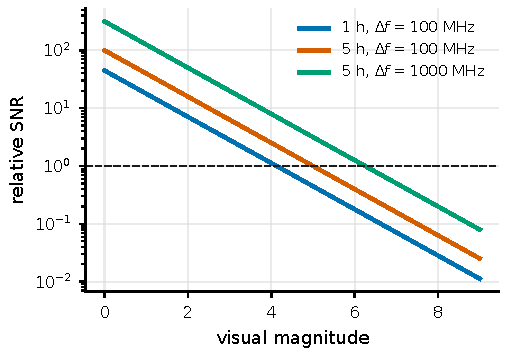
\includegraphics[width=0.86\linewidth]{figures/generated/chapter_05/ch05_snr_scaling.pdf}
\caption{强度干涉信噪比的相对标度。恒星每暗 1 等，光子谱流量约降为原来的 0.398；积分时间和电子带宽只按平方根改善 SNR。曲线未包含收集面积、效率、背景稀释和 \(|V|^2\)，显示亮星选择和高速电子学怎样限制可达信噪比。}
\label{fig:ch05-snr-scaling}
\end{figure}

背景光以两种方式伤害观测。它先增加 shot noise，又把式 \eqref{eq:ch05-correlation-model} 的振幅乘上 \(f_1f_2\)。若每台望远镜里目标光子只占总光子的 70\%，相关振幅已经降到约 0.49。要恢复同样显著性，需要更长积分，并且系统误差更容易占主导。月光、夜天光、PSF 过宽、相邻星污染和探测器暗电流都以这种方式进入。Le Bohec 和 Holder 估算过，Cherenkov 望远镜 \(0.05^\circ\) 量级的光学 PSF 会让夜天光成为暗星灵敏度边界；现代 VERITAS 分析也要修正 night-sky background 和暗电流，否则角直径可产生约 10\% 量级偏差 \citep{2006ApJ...649..399L,2020NatAs...4.1164A,2025ApJ...995..191A}。

系统相关比白噪声更危险，因为目标信号本来只有 \(10^{-6}\) 到 \(10^{-3}\)。常见检查包括：远离零延迟的相关是否为零；互换通道或人为时间偏移后峰是否消失；不同望远镜对、不同夜晚、不同月距和不同电子链路是否给出一致的 \(N_0\)；同一目标的 \(|V|^2\) 是否随投影基线而不是随 PMT 电流、温度或电子增益变化。MAGIC-SII 采用常规相机像素、窄带滤光片、VCSEL 模拟光纤传输、约 110 MHz 聚合带宽和 GPU 实时无死时间相关器，报告了 22 个恒星直径测量；这类系统把限制推向工程稳定性和校准体系，望远镜面积只是其中一项 \citep{2024MNRAS.529.4387A,2022SPIE12183E..0DK,2019ICRC...36..740M,2019ICRC...36..714K}。

\begin{figure}[tbp]
\centering
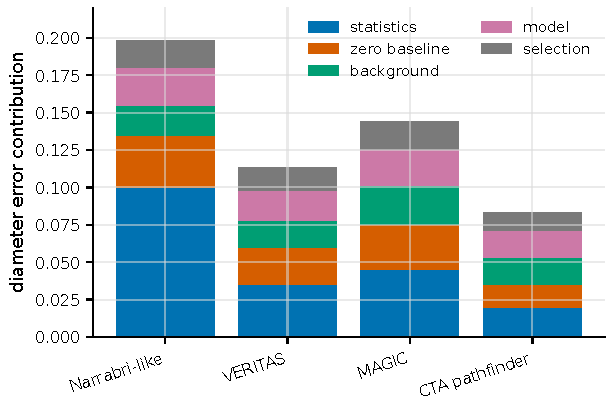
\includegraphics[width=0.82\linewidth]{figures/generated/chapter_05/ch05_error_budget.pdf}
\caption{强度干涉角直径误差预算的组成。统计误差会随光子数和积分时间下降，但零基线定标、背景稀释、恒星模型和天气/选择函数会形成系统误差地板；现代阵列的科学产出取决于这些项能否和 photon noise 一起写进似然。}
\label{fig:ch05-error-budget}
\end{figure}

\section{多基线怎样走向成像}

两台望远镜只能给一个投影基线上的 \(|V|^2\)。若阵列有 \(N\) 台望远镜，同时可形成
\begin{equation}
  N_{\rm base}=\frac{N(N-1)}{2}
  \label{eq:ch05-baseline-number}
\end{equation}
\begin{formulaexplain}
\(N_{\rm base}\) 是可同时形成的望远镜对数；\(N\) 是望远镜数量。每一对望远镜给一条基线，所以基线数随阵列规模近似按 \(N^2/2\) 增长。
\end{formulaexplain}
条基线。强度干涉在这里有一个实际优势：电信号可以复制到许多相关器，形成所有望远镜对，不像振幅干涉那样把同一束相干光分给多个合束器会损失光子。地球自转又会改变每条物理基线的天空投影，使同一望远镜对在一夜中扫过一段 \(u,v\) 轨迹。若每隔几分钟保存一次相关结果，就能把恒星的空间频率采样从几个点扩展成轨迹；多夜、多 hour angle 和多望远镜对一起构成二维 \(u,v\) 覆盖 \citep{2008AIPC..984..205L,2012MNRAS.419..172N,2012MNRAS.424.1006N,2013APh....43..331D}。

\begin{figure}[tbp]
\centering
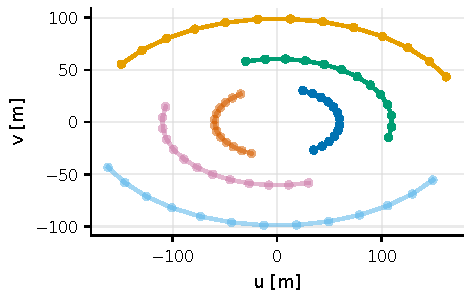
\includegraphics[width=0.82\linewidth]{figures/generated/chapter_05/ch05_uv_coverage.pdf}
\caption{固定望远镜基线在地球自转中投影到不同 \(u,v\) 位置。每条彩色轨迹代表一个望远镜对，负的共轭点也可用于实亮度分布的 Fourier 约束。覆盖越稠密，越能区分圆盘、椭圆、双星和表面斑点。}
\label{fig:ch05-uv-coverage}
\end{figure}

只测 \(|V|^2\) 并不等于只能测直径。对均匀圆盘、椭圆圆盘、双星和 limb darkening 这类低维模型，\(|V|^2\) 已经能给很强约束。若要做模型无关图像重建，则需要补充相位信息或施加图像约束。第 \ref{chap:04} 章的三阶公式 \eqref{eq:ch04-g3-closure} 对应到三台望远镜 \(1,2,3\) 时，项
\[
  2\,{\rm Re}(\gamma_{12}\gamma_{23}\gamma_{31})
\]
含有闭合三角形的相位和。这个量不受单台望远镜相位 piston 的影响，因此在概念上接近振幅干涉的 closure phase。问题是三阶信号比二阶信号弱，光子三元组比光子对少得多，误差传播也更苛刻；它更适合大型阵列和极亮目标，而不是所有观测的默认产品。另一条路线是从二维 \(|V|\) 分布用 Cauchy--Riemann、Gerchberg--Saxton 或 MIRA 等相位恢复与后处理算法重建相位。Nuñez 等人的模拟显示，明亮热星、快速自转星、双星和带表面斑点的恒星在 CTA 类 \(u,v\) 覆盖下可以恢复到有物理意义的形状参数，但结果依赖 SNR、短基线覆盖、先验掩膜和图像正则化 \citep{1966JOSA...56..441G,2012MNRAS.419..172N,2012MNRAS.424.1006N,2014SPIE.9146E..0ZD,2024NJPh...26f3014B}。

从仪器史看，Narrabri Stellar Intensity Interferometer 是第一个完整展示这套方法科学能力的系统。它用两台 \(6.5\,{\rm m}\) 光收集器在 10--188 m 可变基线上工作，滤光片中心约 443 nm、带宽 10 nm，PMT 量子效率约 25\%，有效电子带宽约 60 MHz；1960s--1970s 期间测量了 32 颗恒星的角直径和若干双星系统，最小直径约 \(0.4\,{\rm mas}\) \citep{1967MNRAS.137..375H,1967MNRAS.137..393H,1970MNRAS.148..103H,1971MNRAS.151..161H,1974MNRAS.167..121H,1974MNRAS.167..475H,1974iiia.book.....H}。它后来停用，主要受限于当时的大面积可移动光收集器、低噪声高速电子学和多基线成像能力。

现代 Cherenkov 阵列改变了硬件边界。它们本来为纳秒 Cherenkov 闪光设计，拥有 10 m 级口径、大面积镜面、快速 PMT、长基线和可接受的光学像质。VERITAS 四台 12 m 望远镜已经示范了六条同时基线的强度干涉，\(\beta\) CMa 和 \(\epsilon\) Ori 的直径精度优于 5\%，观测时间只有数小时，并且可在接近满月的非伽马观测时间运行 \citep{2020NatAs...4.1164A}。MAGIC 采用两台 17 m 抛物面望远镜和原有相机像素，系统升级后能在常规伽马观测与 SII 模式之间快速切换，并用 GPU 相关器报告了 22 个恒星直径 \citep{2024MNRAS.529.4387A}。VERITAS 对 \(\beta\) UMa 和 \(\gamma\) Cas 的后续结果把强度干涉从可行性演示推进到具体恒星物理：\(\gamma\) Cas 数据用六条基线和超过 160 pair-hours 观测测得可见 photosphere 的扁率，给出小轴直径约 \(0.43\,{\rm mas}\)、长短轴比约 1.28 和自转轴位置角约 \(116^\circ\) \citep{2024ApJ...966...28A,2025ApJ...995..191A}。

CTAO 的吸引力来自基线和基线数量。公里级基线在 350--450 nm 对应几十微角秒分辨率，几十到上百台望远镜又能带来上千条基线和密集 \(u,v\) 覆盖。它不会替代 CHARA、VLTI 等振幅干涉仪，因为灵敏度、相位和红外能力不同；它更像一个蓝光、超长基线、亮热星和快速变化天体的互补工具。它的科学产出取决于探测器带宽、时间同步、相关器吞吐、背景控制、可复现的零基线校准和面向光学干涉数据标准的数据产品 \citep{2009A&A...507.1719F,2010SPIE.7734E..1CN,2010SPIE.7734E..1TJ,2013APh....43..331D,2014SPIE.9146E..0ZD,2022icrc.confE.803K,2024SPIE13095E..0IT}。

